\chapter{La collection Rondel}


Pour pouvoir être exploitées avec rigueur, toutes ces factures de libraires doivent être envisagées au regard du parcours personnel d'Auguste Rondel, et de la collection qu'elles recensent. 


\section{Parcours personnel d'Auguste Rondel} 

Auguste Rondel (1858-1934) est un banquier français né à Marseille, particulièrement célèbre pour sa vaste collection théâtrale. Sa passion pour la littérature dramatique se manifeste dès l'enfance, et l'amène à constituer sa propre bibliothèque. Sa venue à Paris lorsqu'il intègre l'École Polytechnique lui permet de s'initier au spectacle, et de fréquenter la haute société parisienne. Auguste Rondel est bouleversé par sa découverte des cinq volumes du catalogue de la bibliothèque du marquis de Soleinne, l'un des plus grands collectionneurs de théâtre du XIX\textsuperscript{e} siècle\footcite[Le marquis de Soleinne est l'un des prédécesseurs de Rondel en matière de collection théâtrale, au même titre que les frères Parfaict, premiers grands historiens du théâtre au XVIII\textsuperscript{e} siècle, ou le comte de Pont-de-Veyle, qui constitue à la même époque sa bilbiothèque dramatique.][p. 223-238]{thomas_2005}.
Il s'en inspire donc pour constituer sa collection, et mêle dans cette activité l'érudition du bibliophile et l'esprit de méthode et de rigueur acquis par sa formation. Ce travail est également rendu possible par son sens des relations humaines et grâce au réseau qu'il constitue. A Paris, il est l'ami, le mécène et le conseiller de gens de théâtre, qui l'aident à comprendre ce monde. En région, il organise son réseau de collecte de documents avec l'aide de correspondants bénévoles, et à l'étranger, il entretient une correspondance importante avec des libraires dans différentes villes d'Europe\footcite[p. 239-240]{giteau_2005}.

\begin{figure}[htbp]
    \centering
   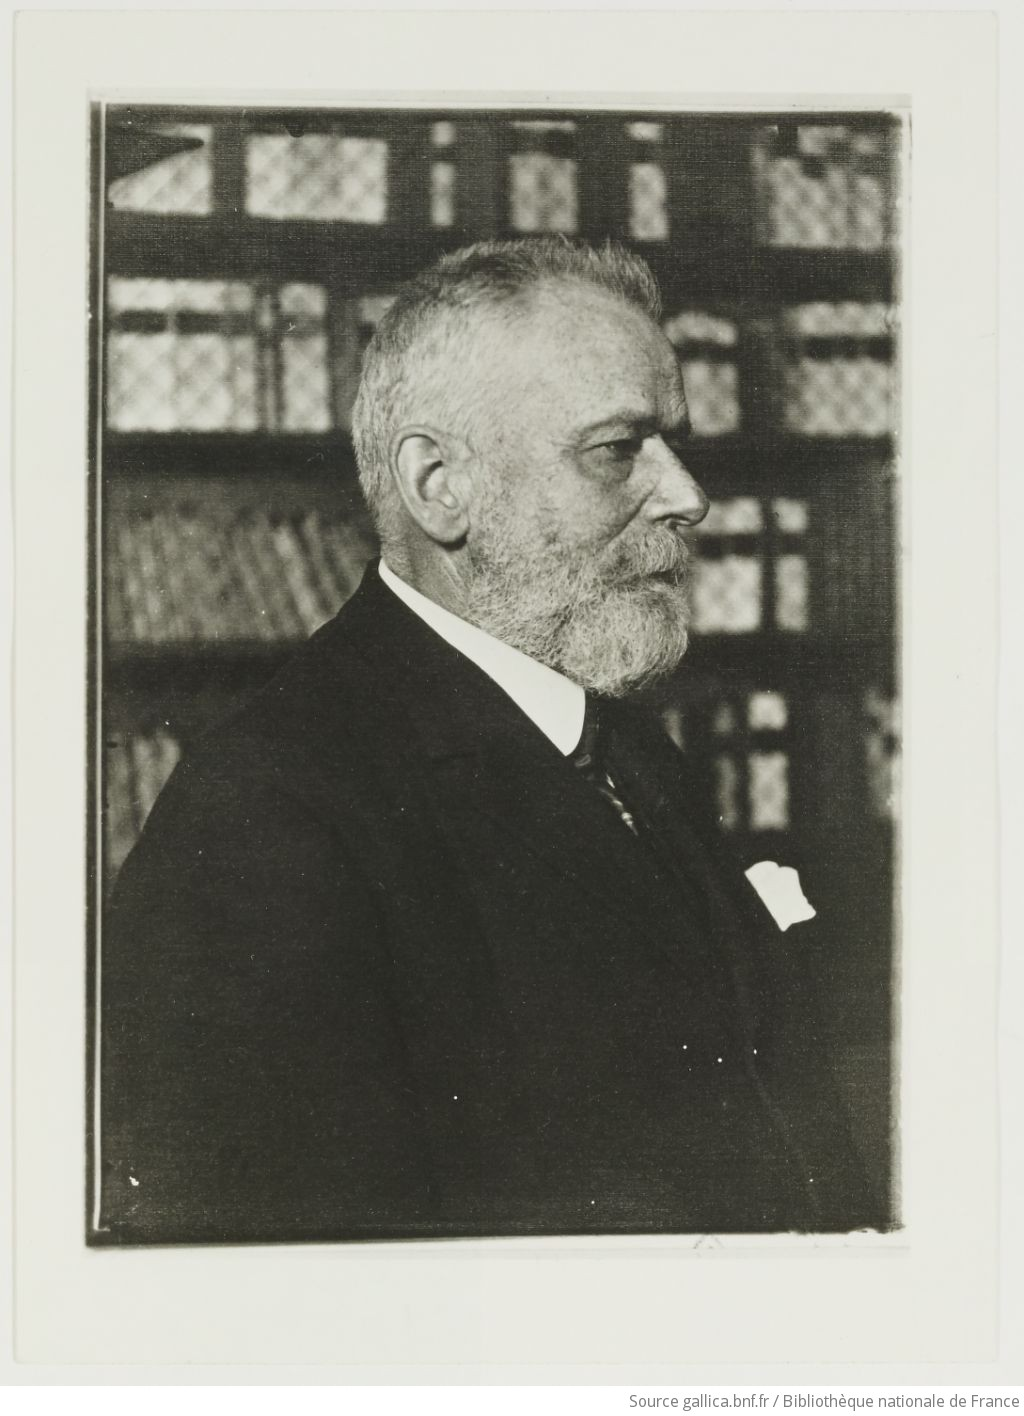
\includegraphics[width=10cm]{Images/rondel_portrait.jpeg}
    \caption{Portrait d'Auguste Rondel, (\enquote{Collection théâtrale Auguste Rondel. 1 - A Marseille et au Palais-Royal}, BnF ASP, 8-RT-3607(1)).}
    \label{fig:portrait-rondel}
\end{figure}

\begin{figure}[htbp]
    \centering
    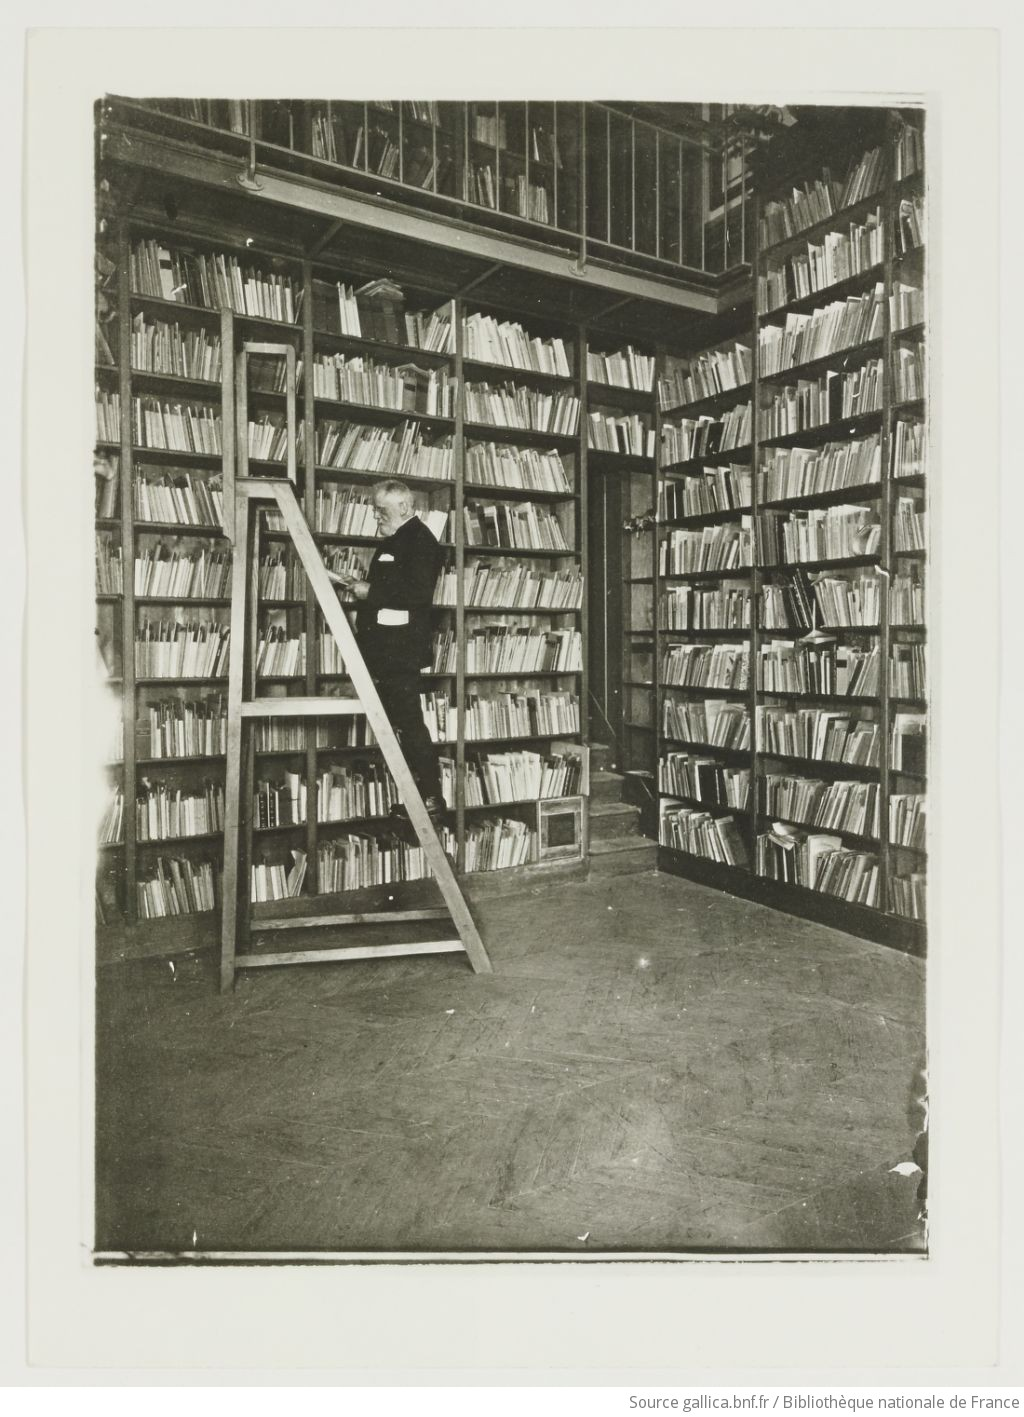
\includegraphics[width=10cm]{Images/RondelBibli2.JPEG}
    \caption{Auguste Rondel dans la salle des auteurs dramatiques du XX\textsuperscript{e} Siècle, (Comédie-française, Palais Royal, 1925), (\enquote{Revue d'histoire du théâtre}, 1958/IV, BnF ASP, 8-RT-3607(13)). }
    \label{fig:rondel-salle-auteurs}
\end{figure}


\section{Composition de la collection}

La collection Rondel regroupe des ouvrages de natures multiples, son fondateur étant \enquote{guidé par une vision encyclopédique et humaniste}\footcite[p. 265]{christout_2005}. Elle réunit de façon à la fois thématique et historique des manuscrits d'auteur, de la correspondance, des relevés de mise en scène, des notes de régie, des éditions rares, ou encore des affiches, des programmes ou des périodiques. Elle est également composée de documents iconographiques, tels que des estampes, des dessins ou des photographies. Rondel rejetait tout a priori, et s'intéressait, au-delà de tout clivage idéologique ou disciplinaire, à tous les genres. 
Son inventaire méthodique nous renseigne plus précisément sur la composition de la collection, dont voici les différentes sections : 


\vspace{1.5cm}

% Tableau en deux colonnes pour décrire la composition de la collection Auguste Rondel
\begin{tabular}{c|c}
\hline
  cote & section\\
\hline
  Ra & Fêtes\\
\hline
  Rae & Estampes : fêtes, spectacles de cour\\
\hline
  Re & Théâtre étranger\\
\hline
 Rf & Théâtre français\\
\hline
 Rj & Périodiques, mémoires, histoires littéraires\\
\hline 
 Rk & Cinéma\\
\hline 
 Ro & Musique\\
\hline 
 Rt & Histoire du théâtre\\
\hline
\end{tabular}

\vspace{1.5cm}


Dans la collection Rondel se trouve une forme particulière de document, créée par Rondel lui-même, qui consiste en un assemblage de coupures de presse sous forme de recueil, consacré à un sujet, une œuvre ou une période. Cette habitude qu'avait Auguste Rondel visait à simplifier la recherche future, en réunissant les sources sur un sujet.\footcite[p. 20]{themis_acrivopoulos_2013}. 

\begin{figure}[htbp]
    \centering
    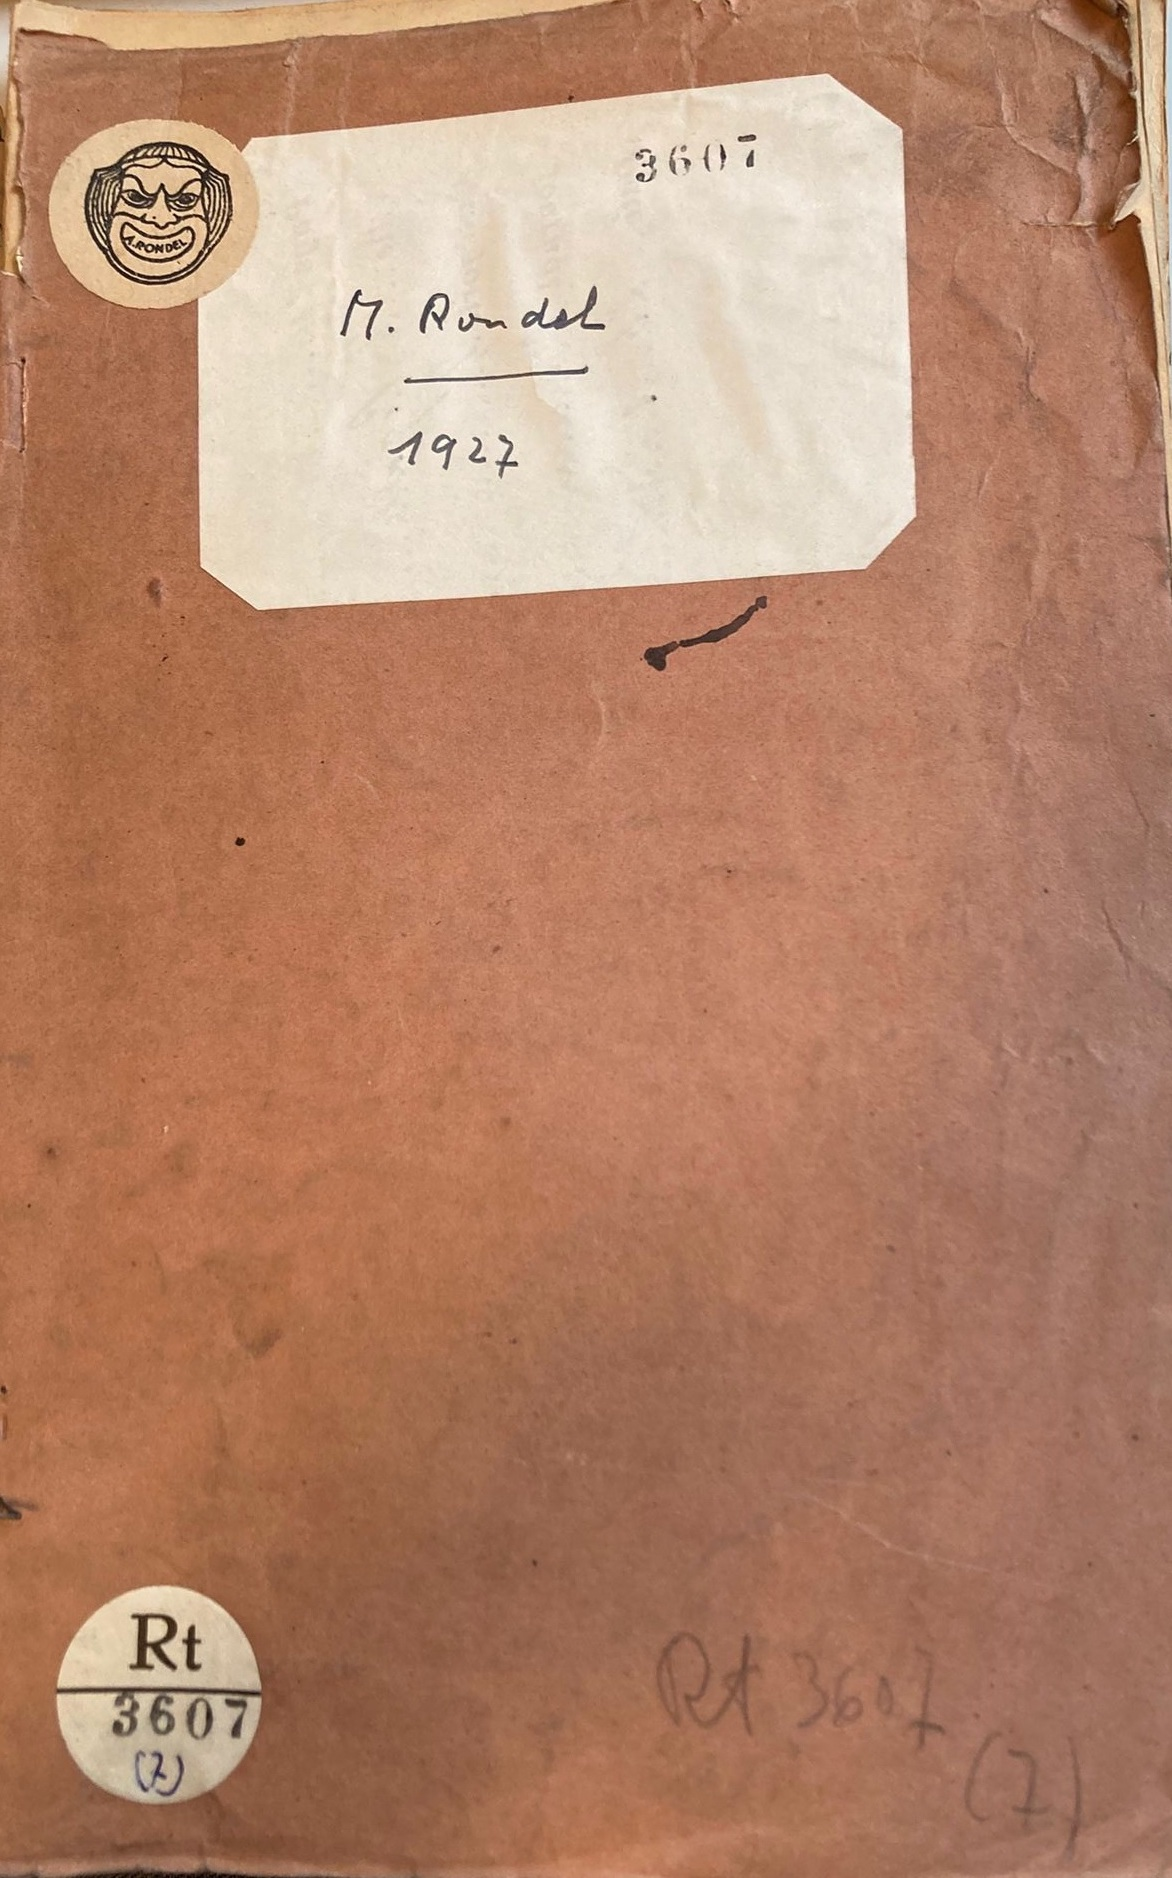
\includegraphics[width=10cm]{Images/RondelRecueilPresse.jpeg}
    \caption{Exemple de dossier de presse issu de la collection Rondel (\enquote{M. Rondel, 1927}, BnF ASP, Rt 3607(7)).}
    \label{fig:dossier-presse-rondel}
\end{figure}

\begin{figure}[htbp]
    \centering
    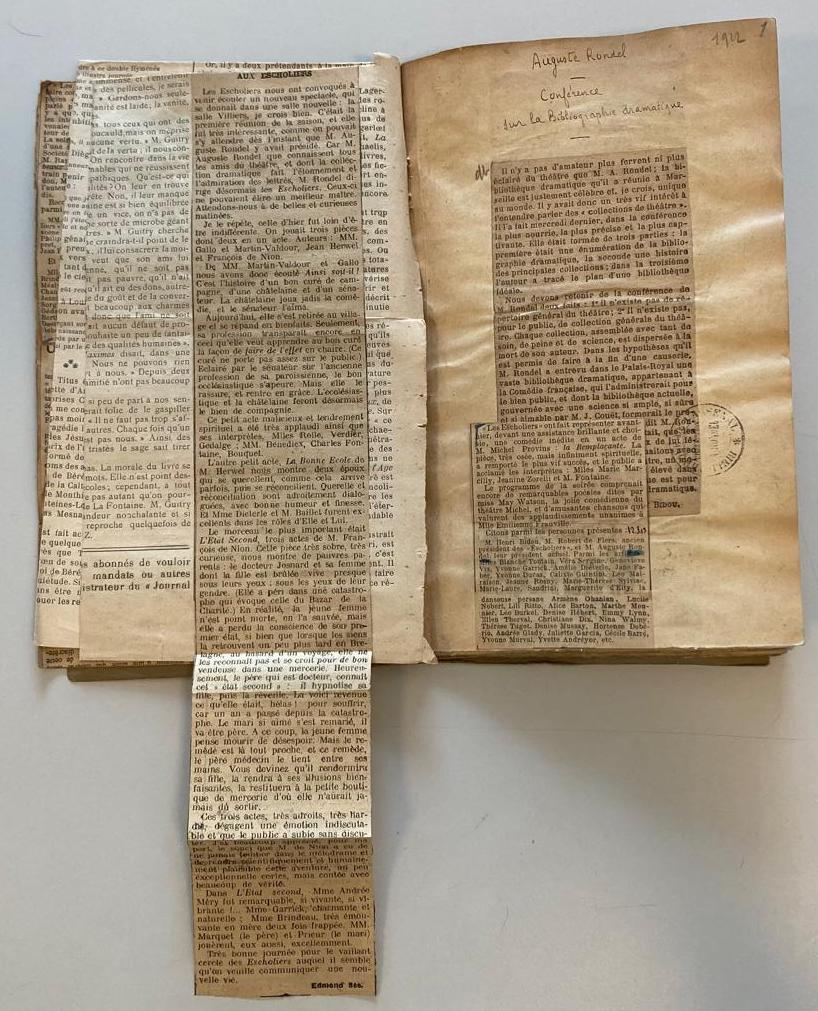
\includegraphics[width=7cm]{Images/RondelRecueilPresse2.jpeg}
    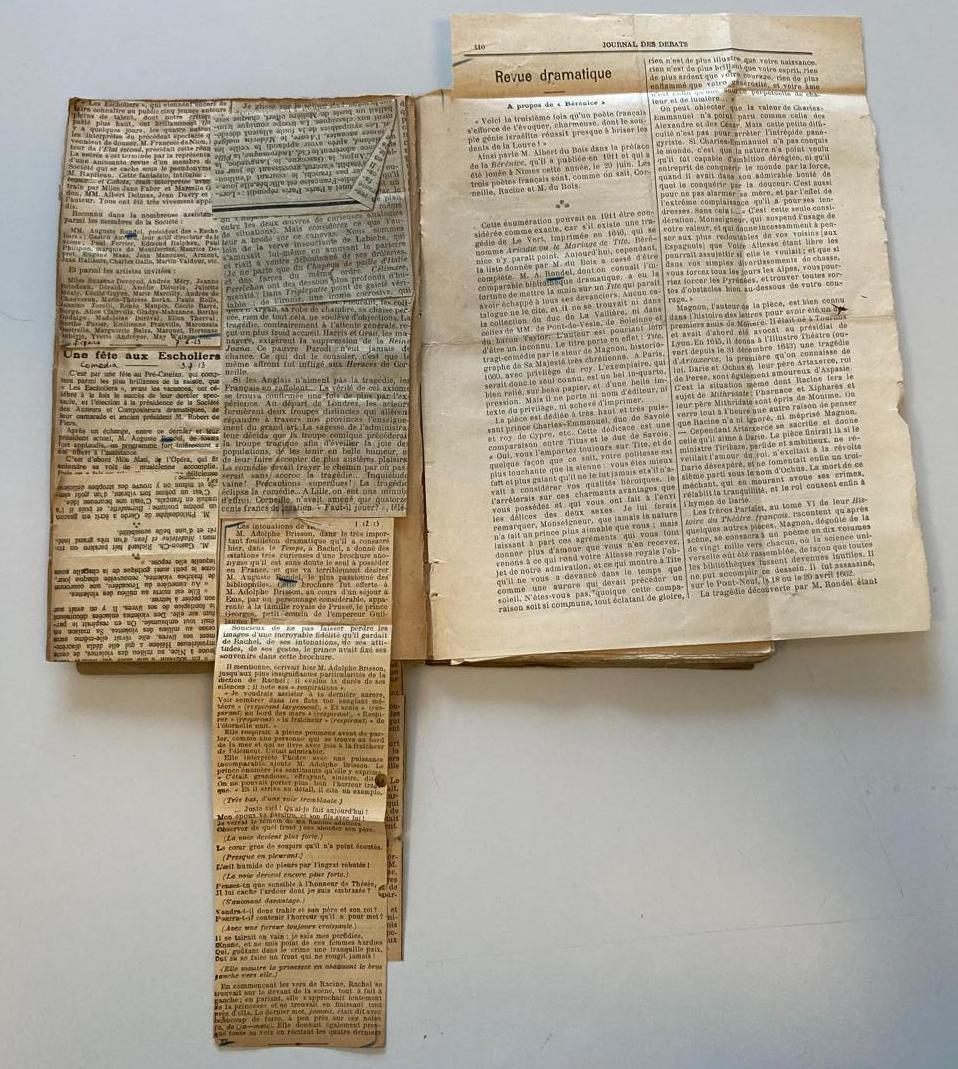
\includegraphics[width=8cm]{Images/RondelRecueilPresse3.jpeg}
    \caption{Coupures de presse, (\enquote{M. Rondel, 1912-1915}, BnF ASP, 8-RT-3607(3)).}
    \label{fig:coupures-presse-rondel}
\end{figure} 


\newpage


Ainsi, la collection constituée par Rondel lui-même compte trois cent mille volumes en 1918, et occupe à cette époque les deux étages de son hôtel particulier sur la place Saint-Ferréol à Marseille. Il consacre l'essentiel de sa fortune à sa collection, soit 7 millions-or en 1914, et lorsqu'il perd ses deux neveux à la guerre, il n'a plus d'héritier direct. Cela expliquerait peut-être en partie pourquoi il a demandé à l'État d'accepter la donation de sa collection et de la mettre à disposition du public à Paris, à la Comédie-Française, donation officialisée en 1920. Cela peut également s'expliquer par le fait qu'il redoutait que sa collection soit dispersée, comme l'ont été certaines bibliothèques théâtrales antérieures\footcite[Parmi ces collections dispersées, on peut citer celle de Charles Nodier en 1830 et 1844, celle de René-Charles Guibert de Pixerécourt en 1839, ou celle en 1864 de Charles-Simon Favart, créateur de la comédie musicale][p. 236]{thomas_2005}. Des crédits d'installation sont votés par la chambre en 1921, et l'inauguration a lieu en 1922. Dans ces nouveaux lieux, Rondel s'occupe de l'administration de sa collection, qu'il continue à enrichir, avec l'aide de Madeleine Horn-Monval. Née en 1886 et morte en 1972, Madeleine Horn-Monval est une bibliothécaire et historienne française, connue pour avoir été la collaboratrice d'Auguste Rondel et pour avoir administré sa collection\footcite[p. 185-188]{Antonutti_2020}. Après avoir travaillé dans l'enseignement, elle quitte ses fonctions pour assister Auguste Rondel dès 1920, et poursuit cette activité après la mort de Rondel, jusqu'en 1951\footcite[p. 43]{themis_acrivopoulos_2013}. Cependant, en septembre 1925, le ministre de l'instruction publique Anatole de Monzie ordonne à Rondel de quitter immédiatement le Palais-Royal sous prétexte de vouloir y loger à la place l'Institut international de coopération intellectuelle\footcite[p. 239-244]{giteau_2005}. Ce déménagement est d'ailleurs largement commenté par la presse de l'époque, comme en témoigne un dossier constitué par Rondel et consacré à ce  sujet\footnote{\enquote{Collection théâtrale Auguste Rondel. 2 - Transfert à l'Arsenal}, BnF ASP, Rt 3607(2).}.  

\begin{figure}[htbp]
    \centering
    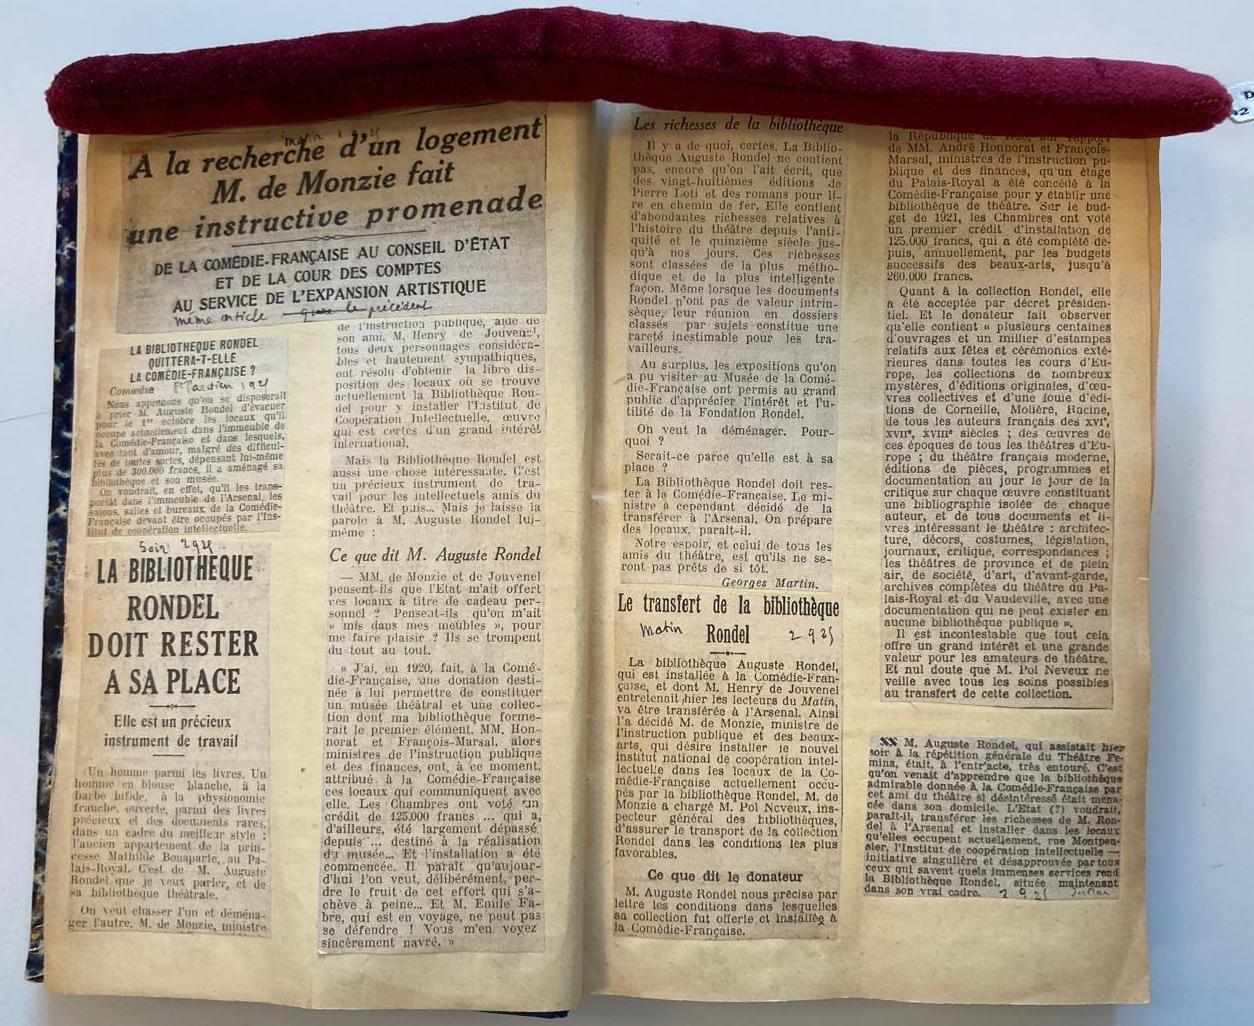
\includegraphics[width=15cm]{Images/coupures_presse_transfert_Arsenal.jpeg}
    \caption{Coupures de presse documentant et protestant contre le transfert à l'Arsenal de la bibliothèque Rondel, (BnF ASP, 8-RT-3607(2)).}
    \label{fig:transfert-arsenal}
\end{figure}


\section{Les archives d'Auguste Rondel, corpus utilisé dans le cadre de mon stage}

Le corpus documentaire utilisé dans mon stage est tiré des \enquote{Archives Rondel}, archives issues de l'activité d'Auguste Rondel et de Madeleine Horn-Monval. 
Les \enquote{Archives Rondel} sont constituées de la correspondance entretenue par Rondel, mais aussi des factures de près de 450 librairies auprès desquelles il a acheté des documents pour enrichir sa  collection entre 1900 et sa mort en 1934\footcite[p. 17-20]{bonicel_2006}. Ces factures proviennent surtout de France, Italie, Allemagne, Autriche, Pays-Bas, Belgique, Angleterre et Suisse. La mission principale de mon stage porte exclusivement sur ces factures, qui occupent une vingtaine de boîtes Cauchard de format quarto, dont l'épaisseur est de 8cm et occupant 1,60 mètres linéaires. 


\begin{figure}[htbp]
    \centering
    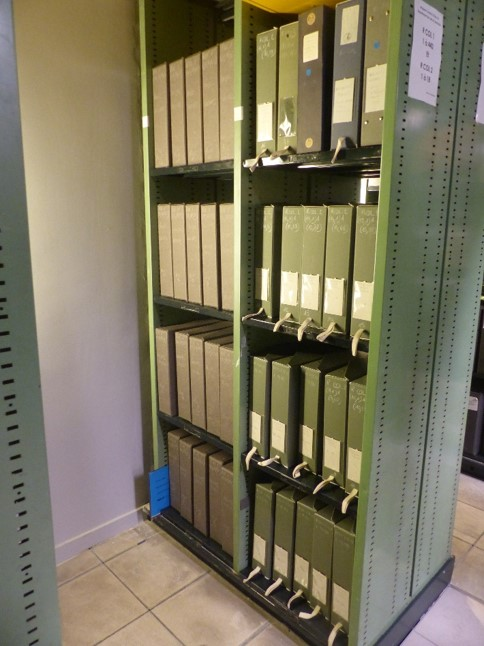
\includegraphics[width=10cm]{Images/boites_factures.jpeg}
    \caption{Factures Rondel, contenues dans les boîtes grises (étagère de gauche).}
    \label{fig:boites-factures}
\end{figure}


Nous nous sommes plus précisément concentrés sur un échantillon représentatif de ce corpus, composé de trois boîtes de factures sélectionnées par mon encadrante scientifique Hélène Keller. Les factures Rondel sont dans le catalogue BnF archives et manuscrits sous la cote RCOL, et chaque dossier est, en général, consacré à un libraire. Certains dossiers de factures contiennent également des extraits de correspondance entre le libraire et Rondel, qui parfois se confondent avec les factures, ou permettent de mieux les comprendre. 

Le type de papier utilisé dans les factures varie beaucoup selon le libraire et l'ampleur du corpus nous empêche d'en distinguer un en particulier. L'échantillon nous permet de dire que l'état de conservation des factures est très bon. Il y a parfois quelques plis et petites déchirures sur les bords de certaines factures, mais cela reste assez rare\footcite{constat_etat}. Les mandats de paiement, qui ont souvent été conservés et sont liés aux factures grâce à des trombones,  sont également en très bon état. Elles sont manuscrites pour la plupart, et le niveau de clarté, de lisibilité et de précision des informations est variable selon le libraire.  

Le nombre de titres écrits par facture varie entre un et une dizaine. Ils correspondent chacun à une ou plusieurs œuvres achetées par Rondel. Certaines factures, à l'image de celle que l'on peut voir ci-dessous, sont très complètes, et renseignent toutes les informations utiles pour identifier une œuvre. D'autres factures sont beaucoup moins détaillées, et ne contiennent que les informations les plus basiques, comme l'auteur, le titre et le prix. Il n'est parfois même pas possible d'identifier l'œuvre tellement le degré d'information est pauvre sur certaines factures. 

\begin{figure}[htbp]
    \centering
    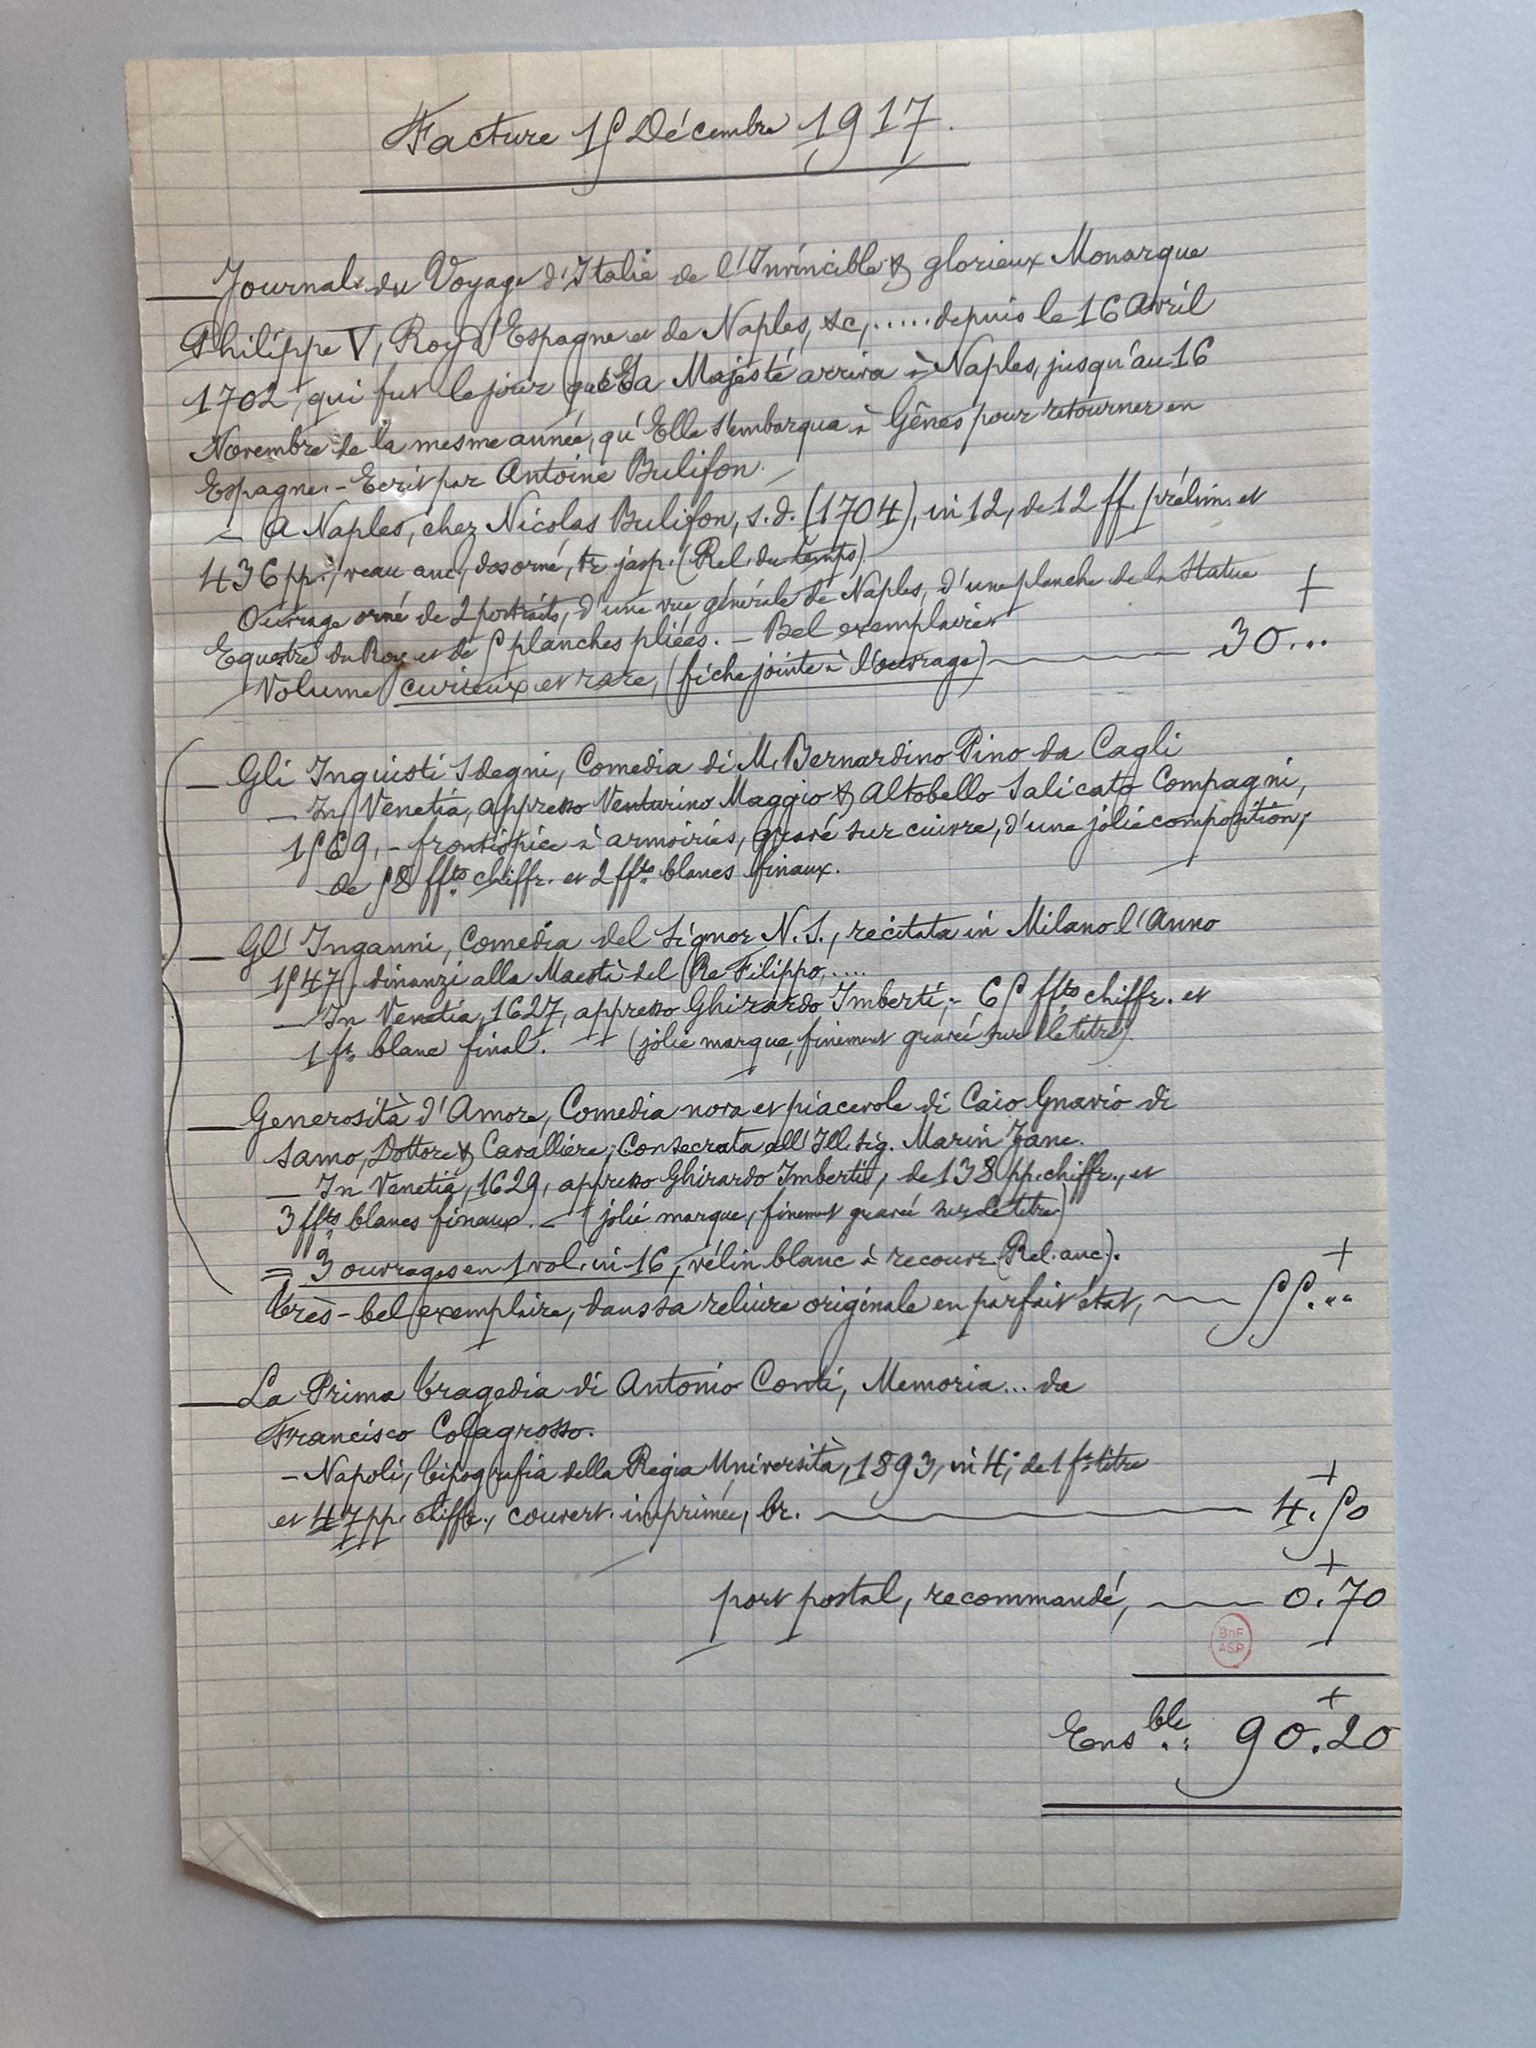
\includegraphics[width=10cm]{Images/Hermal_3.jpeg}
    \caption{Voici un exemple de facture dense et ordonnée : la facture Hermal du 15 décembre 1917 (BnF ASP, RCOL-1(220)).}
\end{figure}


Ainsi ont pu être introduits le parcours personnel d'Auguste Rondel et la constitution de sa collection, que notre projet de base de données a pour but d'étudier. Enfin, la présentation des archives d'Auguste Rondel, en particulier de ses factures, nous a permis de saisir l'ampleur et l'hétérogénéité du corpus à exploiter en vue de la modélisation de cette base.